\begin{table}
\tbl{Comparison of clustering algorithms with a sample of 40000 probe requests}
{\begin{tabular}{lcc} 
	\toprule
	 Algorithm					& Time (s) 	& MAPE (\%) \\
	\midrule
	 Quantile					& 0.002 	&  27 \% \\
	 K-Means			 		& 0.007 	& -23 \% \\
	 Hierarchical Clustering	& 172.520 	&  -9 \% \\
	 Bagged Clustering 			& 0.135 	& -30 \% \\
	 Fisher 					& 3.034 	& -30 \% \\
	 Jenks Natural Break 		& 556.279 	& -30 \% \\
	 \bottomrule
\end{tabular}}
\label{classification-table}
\end{table}

To start, we designed a small pilot study to validate the filtering and
clustering methodology against the scale and complexity of data collected in an
open public area such as a retail high street. We also aimed to find the
algorithm which was best suited for the classification of signal strengths as
'low' and 'high' in order to filter out the background noise. The data was
collected at Oxford Street, London on 20 December 2017 from 12:30 to 13:00 hrs,
Wi-Fi probe requests were collected using the sensor described in Section
\ref{methodology} and pedestrian footfall was manually recorded using the
Android app - Clicker \citep{bala2018clicker}. Being located at one of the
busiest retail locations in the United Kingdom, the Wi-Fi sensor captured
approximately 60,000 probe requests during the half hour period; 3,722 people
were manually recorded walking on the pavement during that time. The surveyor
positioned himself at the front of a store while carrying the sensor in a
backpack and counted people walking by the store on the pavement (3m wide
approximately) using a mobile phone. The sensor was kept as close to the store
window as possible, and the manual count was done as a cordon count in front of
the store.

As a first step we aggregated the probe requests by their MAC addresses for
every minute to generate a minute by minute count of the number of people near
the sensor. We assumed that each MAC address corresponded to a mobile device and
hence a pedestrian. We then compared this preliminary `footfall' count to the
actual number of pedestrians recorded manually to check for it's robustness. We
used Mean Absolute Percentage Error (MAPE) as a measure of robustness of the
count, since it provided a simple and quick measurement and the street
conditions ensured that there are no intervals without any footfall. We found
that the MAPE in the raw counts compared to the ground truth was around 425\%.
This suggests the presence of large amount of noise in the data which may have
been generated by the sources of uncertainties discussed in Section
\ref{methodology} thus demonstrating the need for filtering the data.

We then classified the probe requests as `high signal strength' and `low signal
strength' using various one dimensional clustering algorithms such as k-means,
quantile, hierarchical clustering, bagged clustering, fisher and jenks natural
breaks. The results are shown in Table \ref{classification-table}. We found that
while hierarchical clustering and jenks gave us fairly low errors, they were too
resource intensive for practical use with a larger dataset. We also found that
k-means gave the quickest results with the lowest MAPE, closely followed by
quantile algorithm. The cut-off point or threshold for the collected data with
which we could classify as high and low was -71 dBm. We then removed all the
probe requests which reported `low signal strength' and repeated the same
aggregation process as before to produce footfall count. This process resulted
in a footfall count with a net MAPE of 30\%. Although the results are
encouraging we are still not completely confident that our filtering process is
removing noise or has any correlation the configuration of sensor or position of
the mobile devices. These concerns need to be addressed with a larger survey
with multiple locations of varying orientations.

\begin{figure}
\begin{center}
\vspace{10pt}
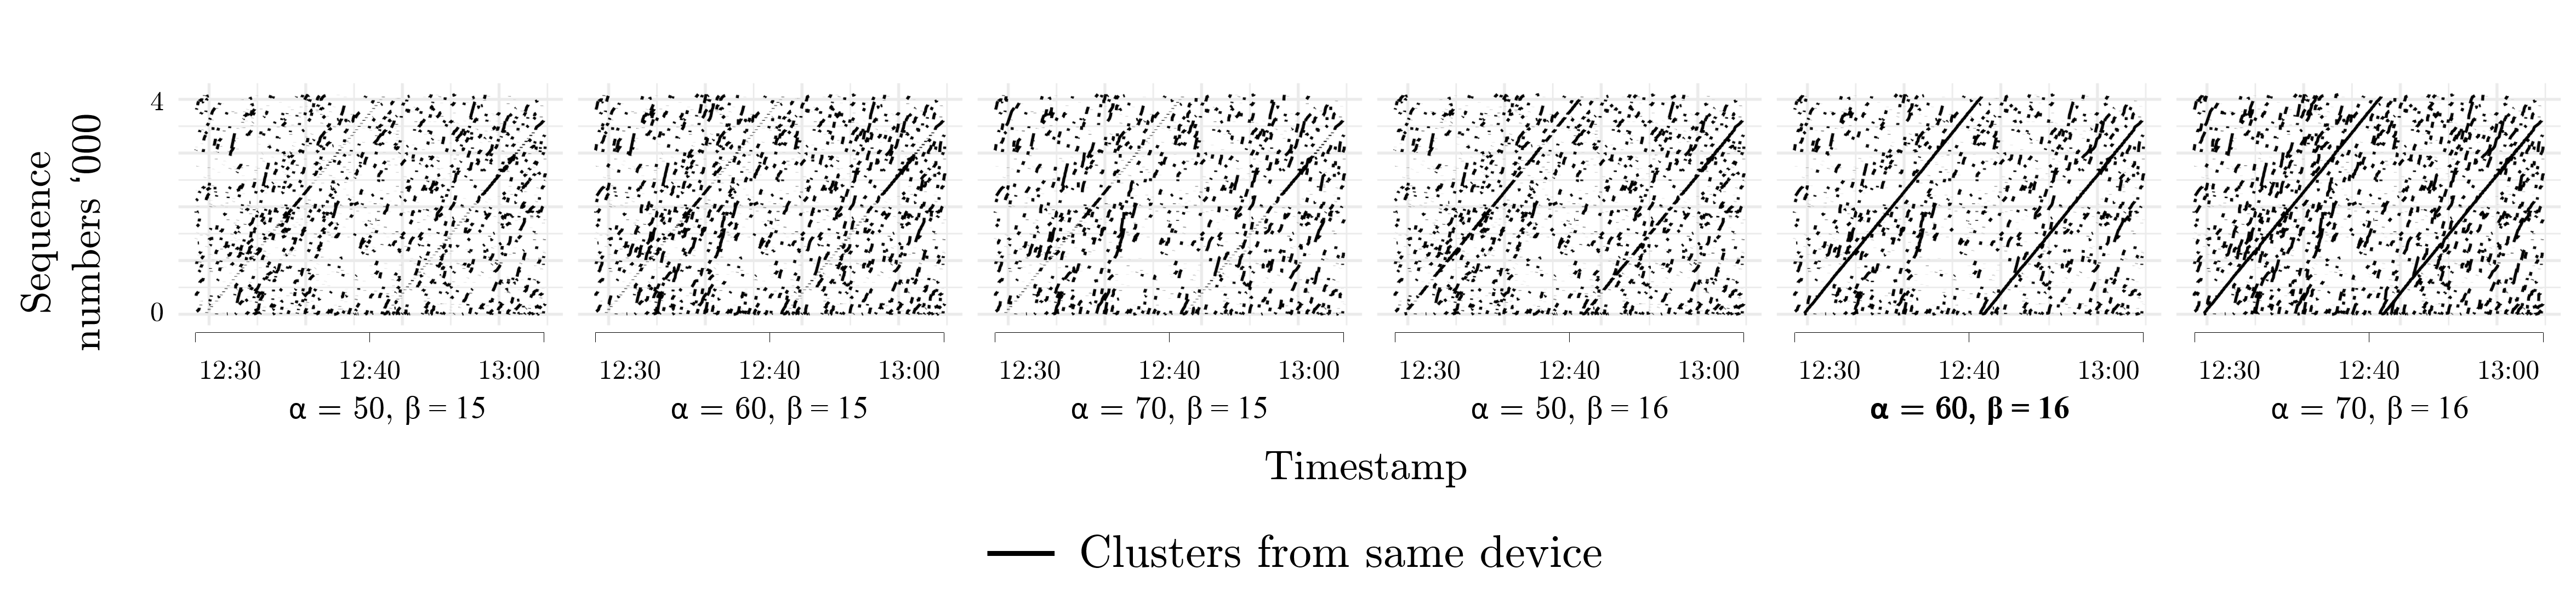
\includegraphics [width=\linewidth,trim=10 30 10 75,clip]
    {images/pilot_clustering_params.png}
\caption{The clustering process was repeated with both increasing sequence
    number threshold ($\alpha$) and time threshold ($\beta$), until we arrived
    at the lowest parameters where the know device (black line) is clustered as
    a single device.}
\label{pilot_clustering_params}
\end{center}
\end{figure}

\begin{figure}
\centering
\subfigure[Clustering probe requests based on increasing sequence numbers 
	present in them.]
	{\resizebox*{0.45\linewidth}{!}
	{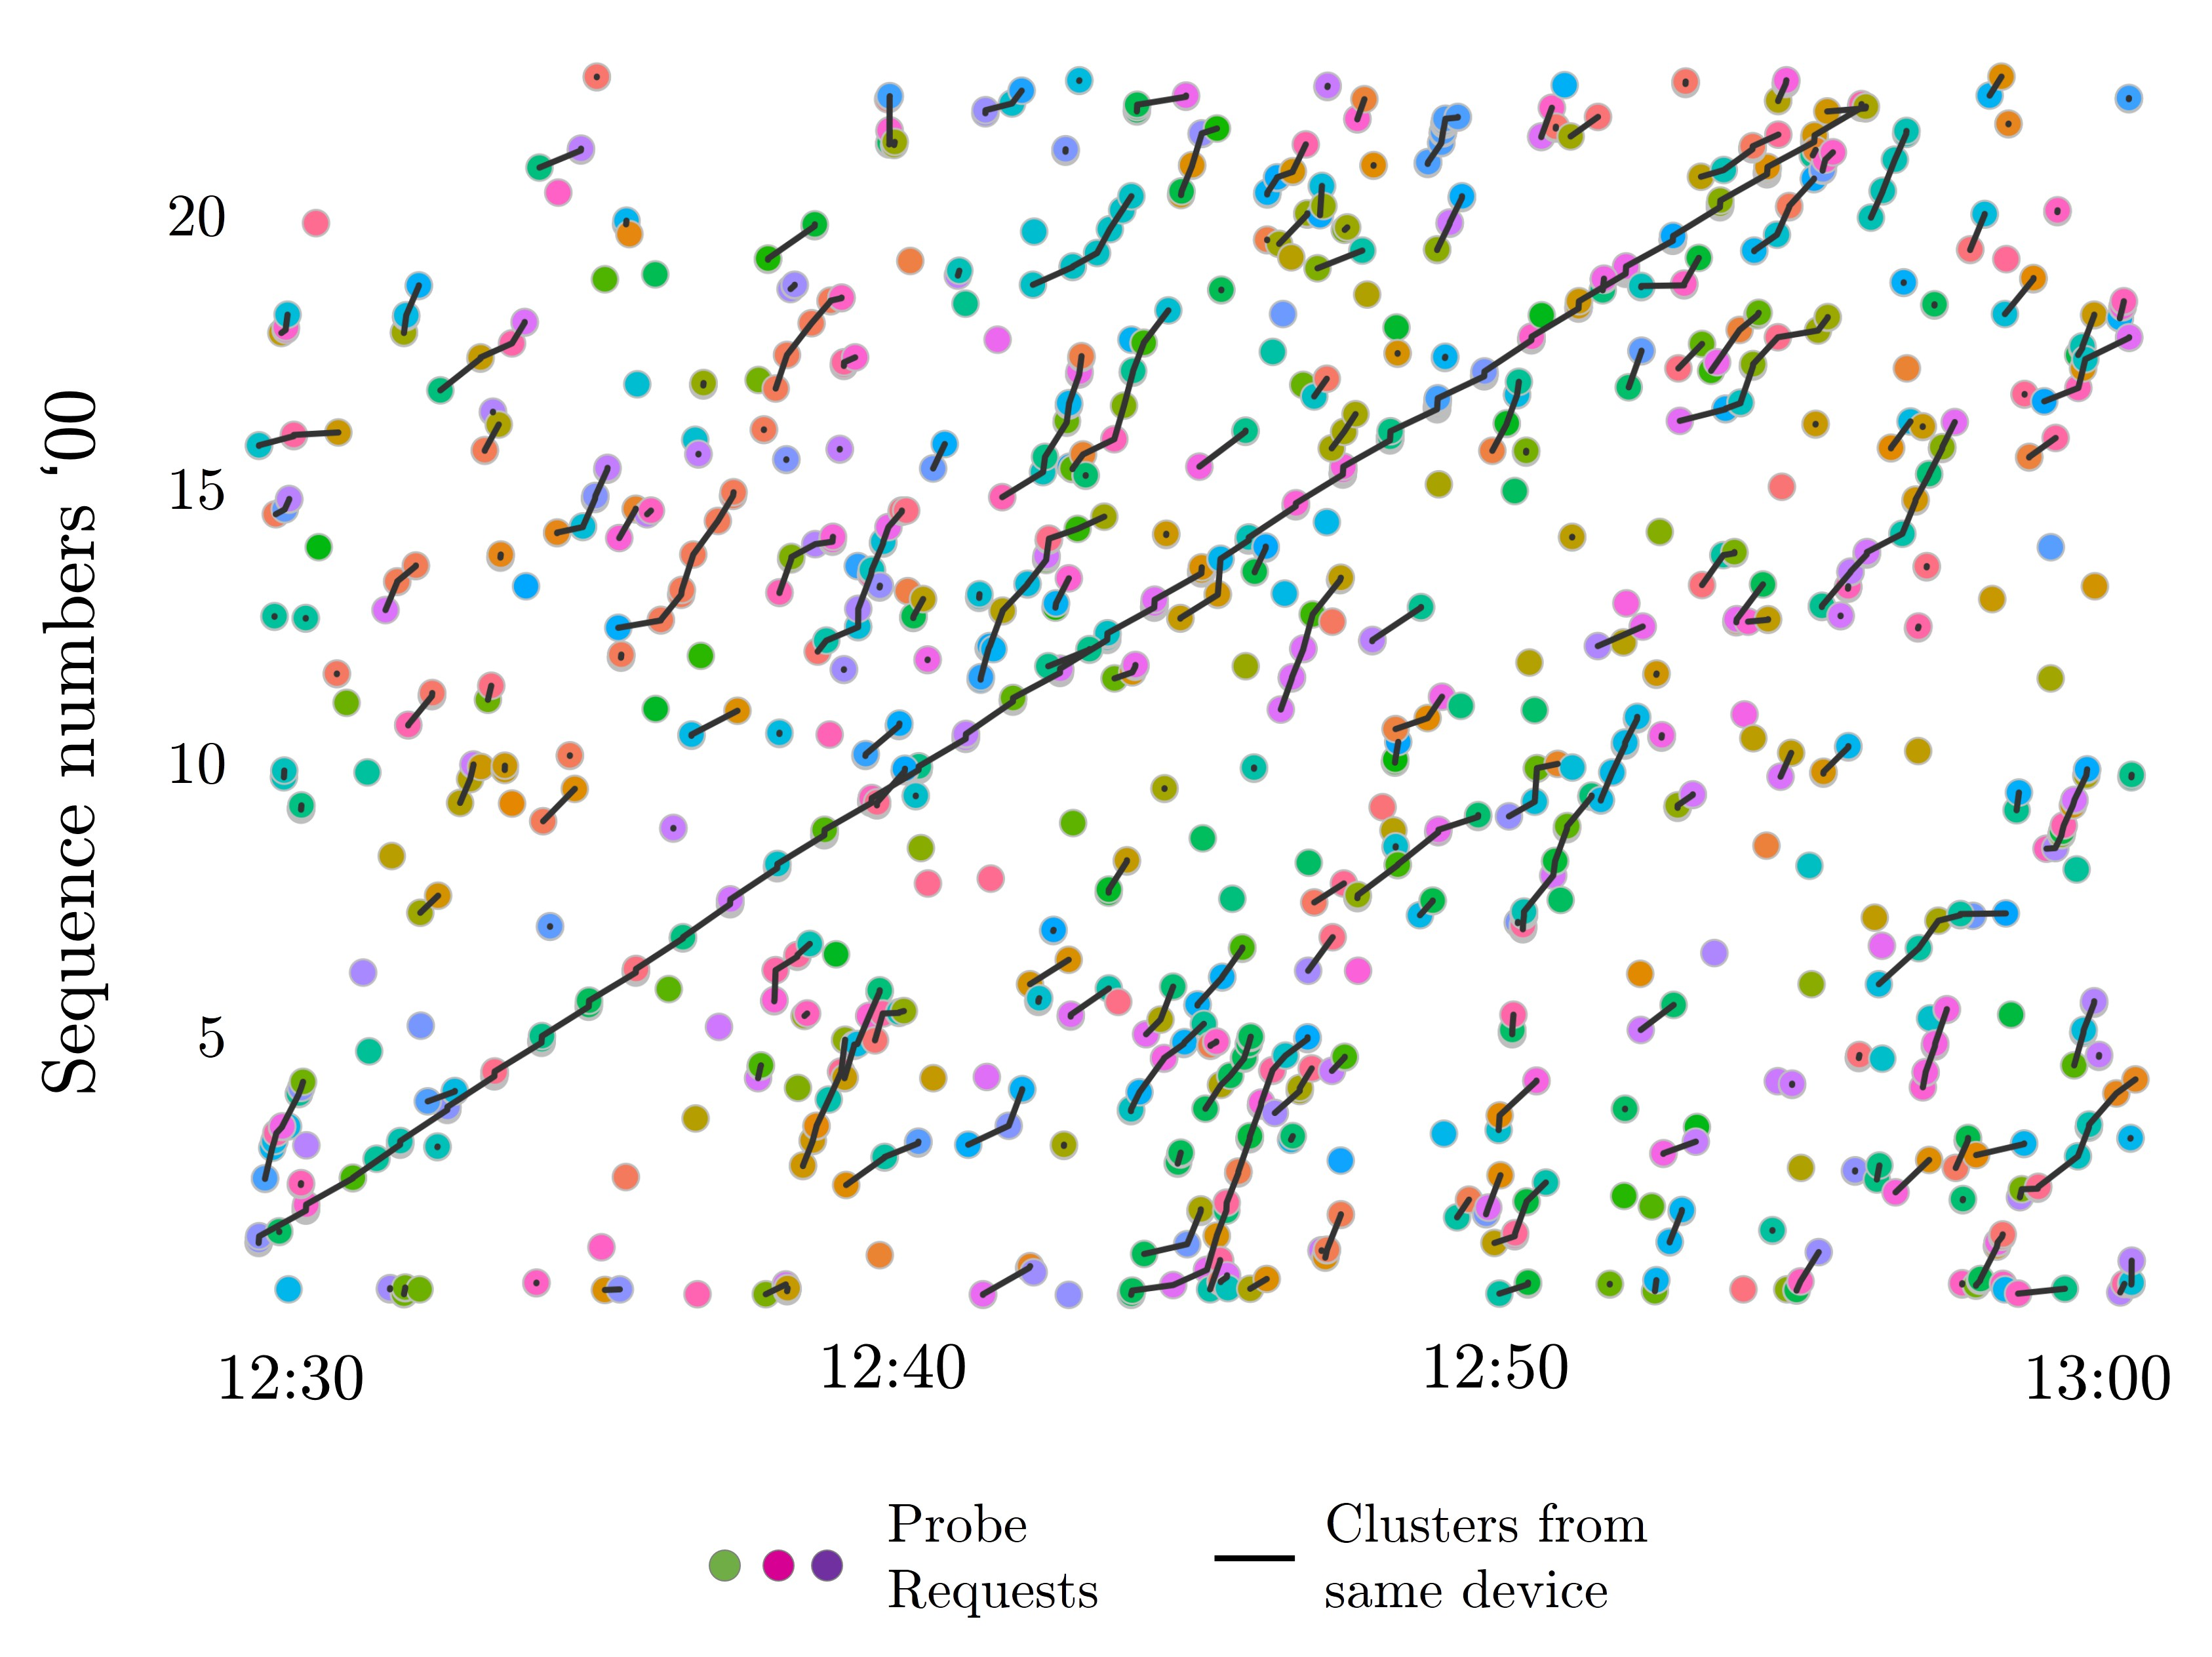
\includegraphics{images/pilot_clustering.jpeg}}}
\hspace{20pt}
\subfigure[Comparison of sensor based counts with the ground truth.]
	{\resizebox*{0.45\linewidth}{!}
	{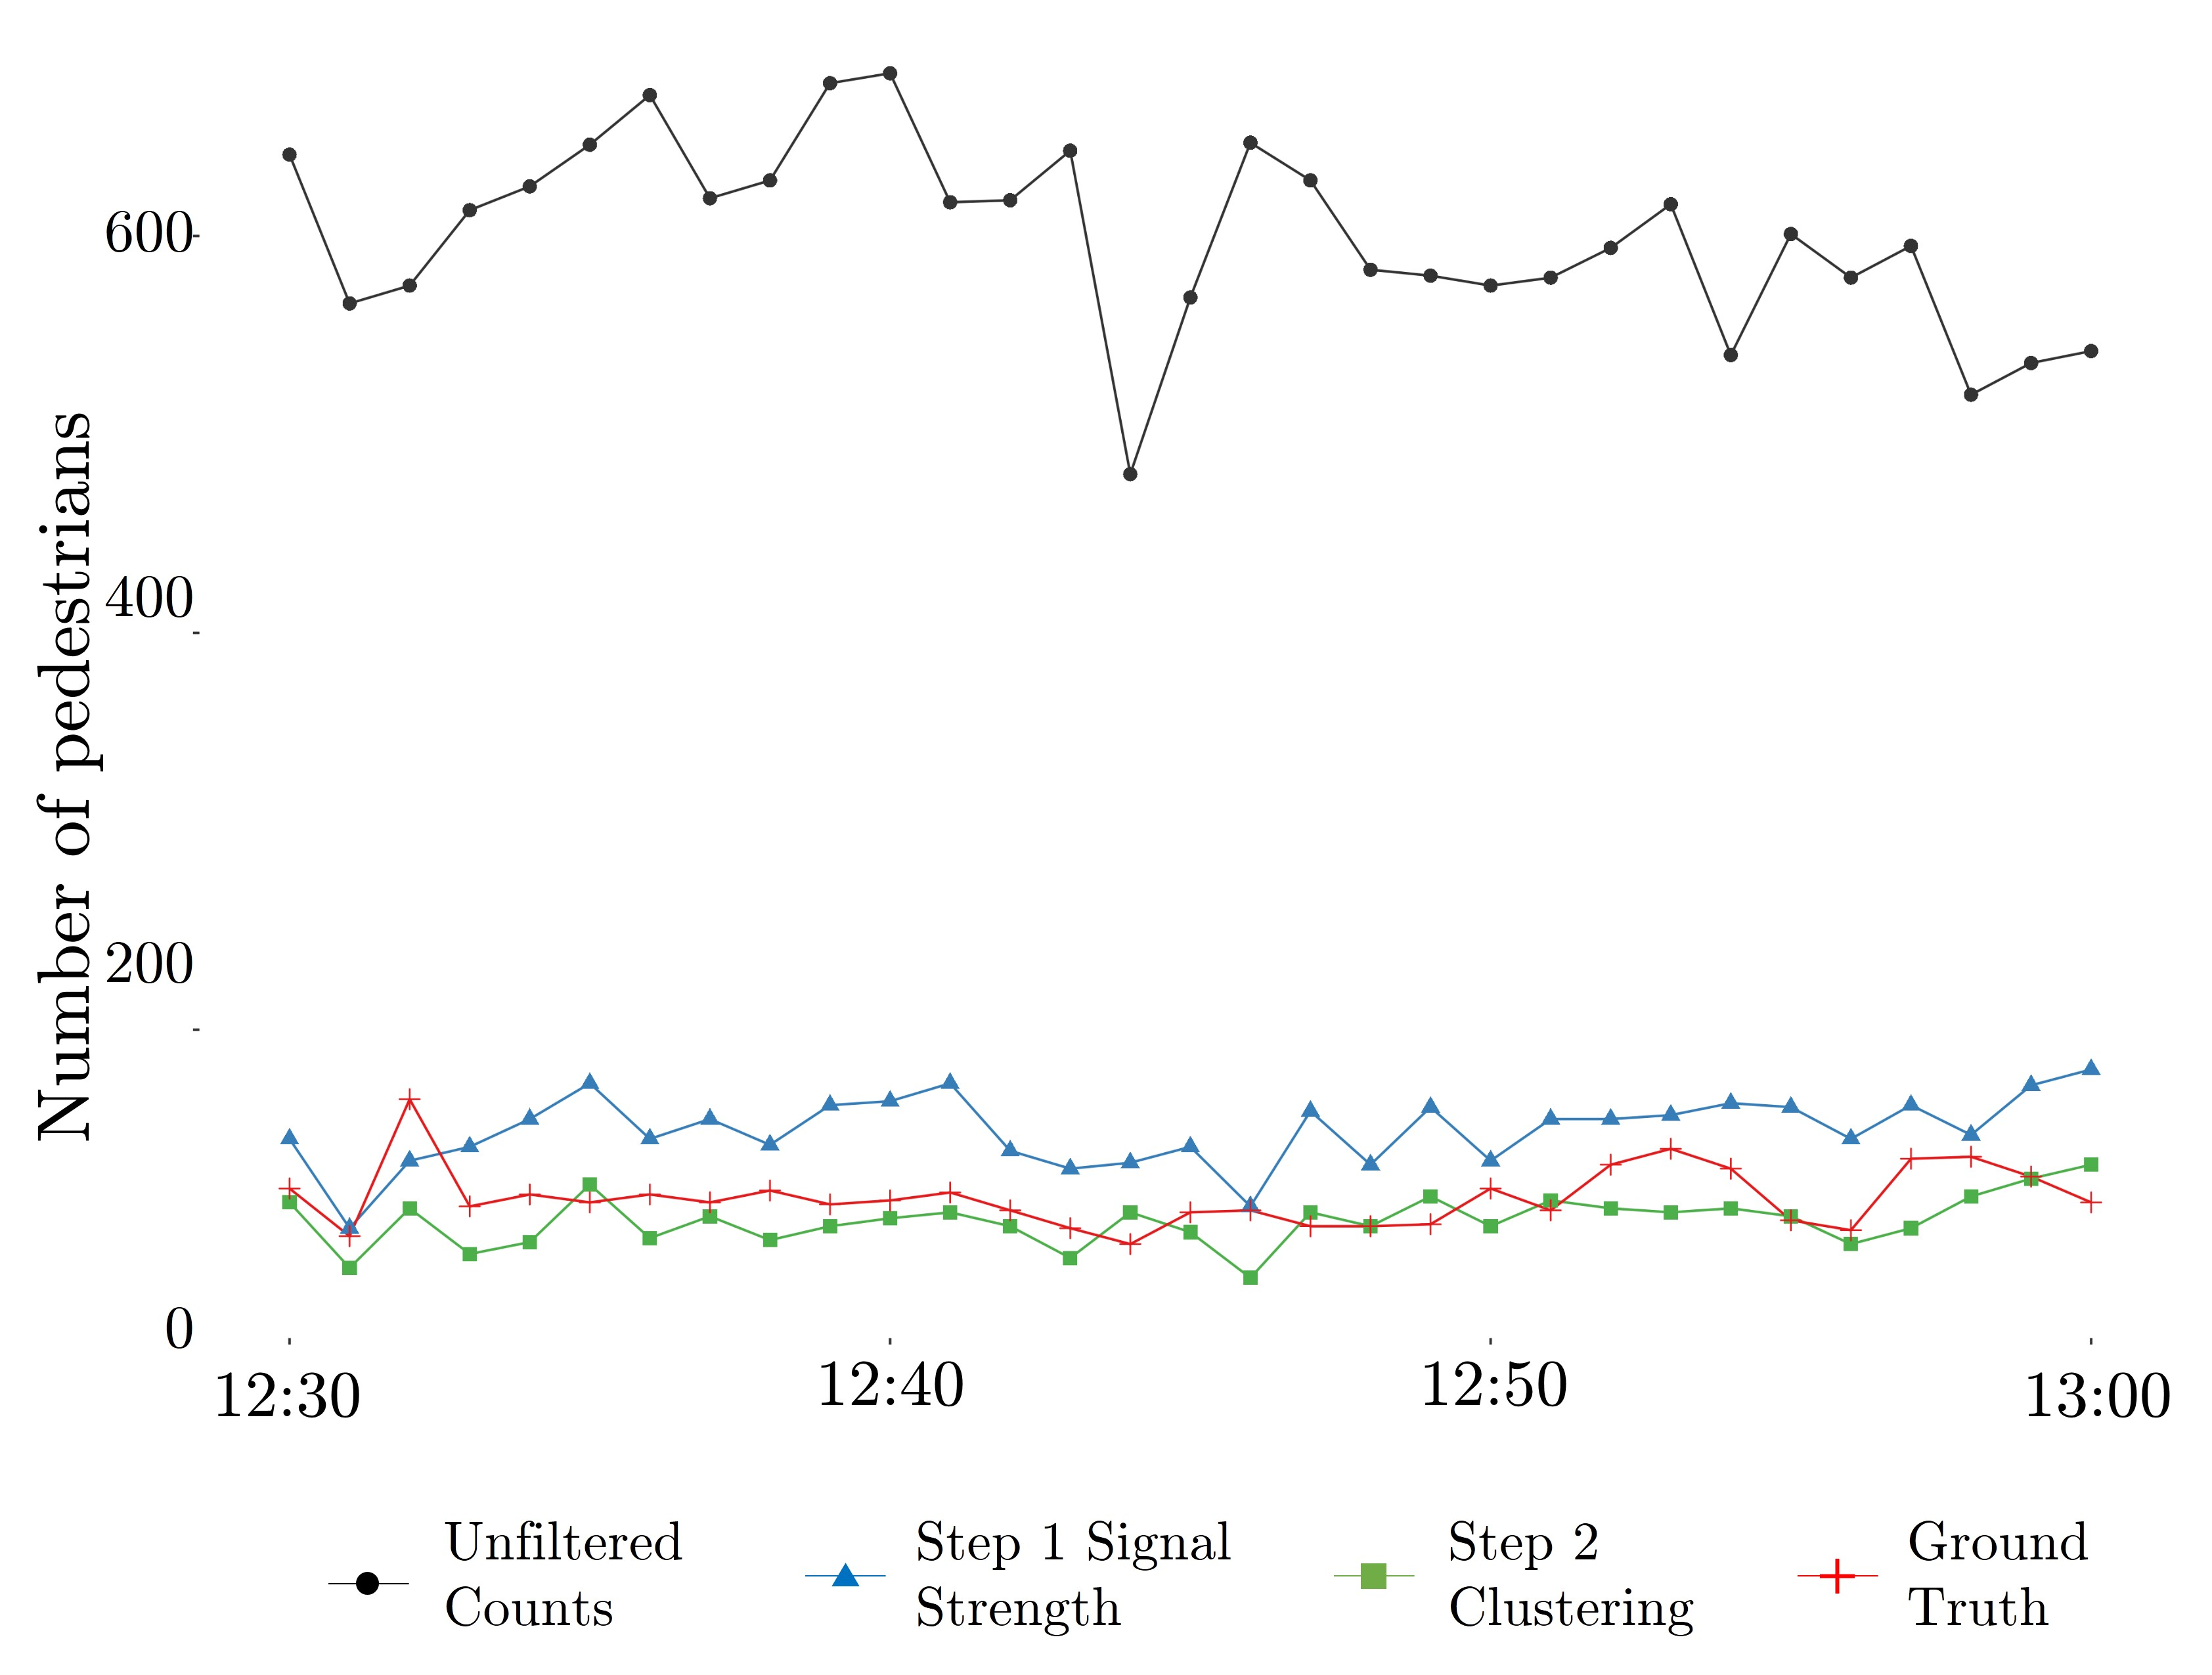
\includegraphics{images/pilot_comparison.jpeg}}}
\caption{The results of the pilot study demonstrating the validity of the
	methodology.} 
\label{pilot_results}
\end{figure}

The next challenge was to identify the probe requests which are generated by the
same device irrespective of the MAC randomisation process. We used the algorithm
defined in Section \ref{methodology} and assigned a unique identifier or
signature to each probe request, independent of their the MAC addresses. Since
we didn't know the nature or frequency of the MAC address randomisation process,
we used the surveyor's mobile device as a reference. As the surveyor's device
was being actively used to count pedestrians and it's Wi-Fi module was kept
active without establishing connection to any network, the device was known to
be continuously probing for new networks. We also knew that the OUI of the
device was 'Google' and the device was regularly randomising it's MAC address,
thus providing us an excellent reference with which we could optimise the
parameters for our clustering algorithm. Using this reference device we observed
that the threshold for time $\alpha$ and the threshold for sequence numbers,
$\beta$ are 16 seconds and 60 respectively via trial and error. This process is
shown in Figure \ref{pilot_clustering_params}. This was undertaken on top the
filtering done based on signal strength, and only for the probe requests with
randomised MAC addresses. Figure \ref{pilot_results} shows the results of this
clustering process on a small set of randomised probe requests. The probe
requests with different randomised MAC address are shown by the coloured points
and the lines joining them show that those probe requests were most likely be
generated by the same device. We finally aggregated the probe requests as we did
before but with the device signature rather than MAC addresses. This results in
a footfall count with a MAPE of -18\% compared to the manual count. A comparison
of minute by minute counts resulting from different filtering processes along
with the ground truth is shown in Figure \ref{pilot_results} illustrating the
promising effectiveness of the methods.

To conclude, from the pilot study we found that both the filtering and the
clustering methods we devised worked on complex real world data and resulted in
final pedestrian counts within a MAPE of 20\%. We also found that `k-means' and
`quantile' are best algorithms for clustering signal strengths. Finally, we
observed that the best thresholds for time and sequence numbers in the
clustering algorithm is around 16 and 60 respectively.
